\documentclass[coursework]{SCWorks}
\usepackage[hidelinks]{hyperref}
\usepackage[T2A]{fontenc}
\usepackage[utf8]{inputenc}
\usepackage[english,russian]{babel}
\usepackage[sort,compress]{cite}
\usepackage{minted}
\usepackage{graphicx}
\usepackage{preamble}
\usepackage{enumitem}
\usepackage{url}
\usepackage{amsmath}
\usepackage{amssymb}
\usepackage{amsthm}
\usepackage{fancyvrb}
\usepackage{longtable}
\usepackage{array}
\usepackage{tempora}

\setminted[cpp]{
    frame=lines,
    framesep=2mm,
    linenos=true,
    breaklines=true,
    fontsize=\small,
    tabsize=4
}



\begin{document}

\chair{математической кибернетики и компьютерных наук}

\title{Реализация алгоритма симметричного шифрования AES}

\course{1}

\group{111}

\napravlenie{02.03.02 "--- Фундаментальная информатика и информационные технологии}

\author{Терентьева Даниила Витальевича}

\chtitle{доцент, к.\,ф.-м.\,н.}
\chname{С.\,В.\,Миронов}

\satitle{доцент, к.\,ф.-м.\,н.}
\saname{Н.\,С.\,Рыданов}

\patitle{доцент, к.\,ф.-м.\,н.}
\paname{С.\,В.\,Миронов}

\nirtitle{доцент, к.\,п.\,н.}
\nirname{Н.\,С.\,Рыданов}

\date{2026}

\maketitle

\secNumbering

\tableofcontents

\intro

В современном мире защита информации является одной из ключевых задач
информационной безопасности. Для обеспечения конфиденциальности данных широко
применяются алгоритмы симметричного шифрования. Одним из наиболее
распространённых и надёжных стандартов является алгоритм
AES (Advanced Encryption Standard)~\cite{fips197}.

Алгоритм AES был принят Национальным институтом стандартов и технологий
США (NIST) в 2001 году и заменил устаревший алгоритм DES~\cite{fips197}.
AES используется в банковских системах, VPN-сетях, беспроводных протоколах
связи, операционных системах и веб-приложениях.

Основным преимуществом AES являются высокая криптостойкость, производительность
и возможность эффективной реализации как программными, так и аппаратными
средствами~\cite{daemen2002}.

\section{Теоретические основы AES}

AES представляет собой блочный симметричный алгоритм шифрования~\cite{fips197}.
Размер блока данных составляет 128 бит. В зависимости от длины ключа различают
следующие версии алгоритма:

\begin{itemize}[label=\textbullet]
    \item AES-128;
    \item AES-192;
    \item AES-256.
\end{itemize}

В данной работе рассматривается версия AES-128, использующая ключ длиной 128 бит
и 10 раундов преобразований.

Каждый раунд AES включает следующие операции:

\begin{itemize}[label=\textbullet]
    \item \texttt{SubBytes};
    \item \texttt{ShiftRows};
    \item \texttt{MixColumns};
    \item \texttt{AddRoundKey}.
\end{itemize}

Схема выполнения раундов алгоритма AES представлена на рисунке~\ref{fig:aes_scheme}.

\begin{figure}[h]
    \centering
    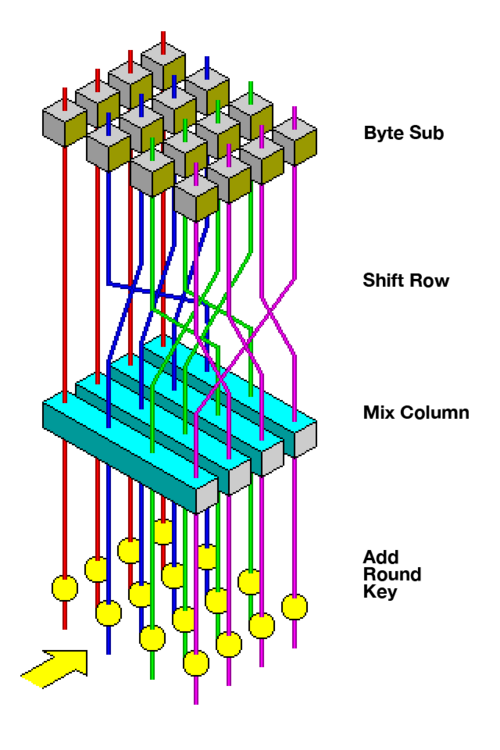
\includegraphics[width=0.75\textwidth]{images/aes_scheme.png}
    \caption{Схема раундов алгоритма AES}
    \label{fig:aes_scheme}
\end{figure}

\section{Математические основы алгоритма AES}

\subsection{Операции в поле \texorpdfstring{GF($2^8$)}{GF(2\textasciicircum 8)}}

AES выполняет вычисления в конечном поле Галуа
GF($2^8$)~\cite{daemen2002}. Каждый байт
интерпретируется как полином степени не выше~7.

Сложение элементов поля выполняется по операции XOR:
\begin{equation}
    a(x) + b(x) = a(x) \oplus b(x)
    \label{eq:xor}
\end{equation}

Умножение выполняется по модулю неприводимого полинома:
\begin{equation}
    m(x) = x^8 + x^4 + x^3 + x + 1
    \label{eq:poly}
\end{equation}

Этому полиному соответствует шестнадцатеричное значение \texttt{0x11B}:
\begin{equation}
    m(x) = \texttt{0x11B}
    \label{eq:hex}
\end{equation}

\subsection{Преобразование SubBytes}

Операция \texttt{SubBytes} выполняет нелинейную замену каждого байта
с использованием таблицы замены S-box~\cite{fips197}.

Преобразование строится следующим образом:
\begin{equation}
    b_i' = A \cdot b_i^{-1} + c
    \label{eq:subbytes}
\end{equation}
где:
\begin{itemize}[label=\textbullet]
    \item $b_i^{-1}$ "--- мультипликативная обратная величина в поле GF($2^8$);
    \item $A$ "--- фиксированная матрица аффинного преобразования;
    \item $c$ "--- константный вектор.
\end{itemize}

Преобразование \texttt{SubBytes} повышает криптографическую стойкость алгоритма
за счёт нелинейности. Таблица замены S-box представлена на
рисунке~\ref{fig:sbox}.

\begin{figure}[h]
    \centering
    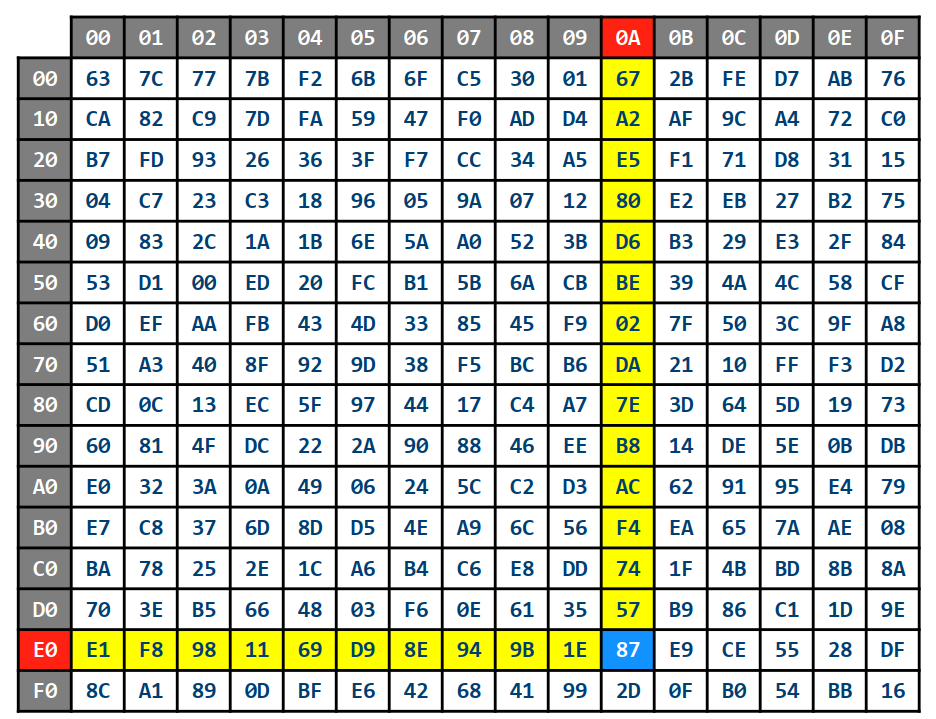
\includegraphics[width=0.85\textwidth]{images/sbox.png}
    \caption{Таблица замены S-box алгоритма AES}
    \label{fig:sbox}
\end{figure}

\subsection{Преобразование ShiftRows}

Операция \texttt{ShiftRows} выполняет циклический сдвиг строк матрицы
состояния влево. Строка с номером~$r$ сдвигается на $r$~позиций~\cite{fips197}:
\begin{equation}
    s'_{r,c} = s_{r,\,(c + r) \bmod 4}, \quad r, c \in \{0, 1, 2, 3\}
    \label{eq:shiftrows}
\end{equation}

Таким образом:
\begin{itemize}[label=\textbullet]
    \item строка~0 не сдвигается;
    \item строка~1 сдвигается на 1~байт влево;
    \item строка~2 сдвигается на 2~байта влево;
    \item строка~3 сдвигается на 3~байта влево.
\end{itemize}

\subsection{Преобразование MixColumns}

Операция \texttt{MixColumns} выполняет перемешивание данных внутри каждого
столбца матрицы состояния~\cite{daemen2002}.

Преобразование описывается следующим выражением:
\begin{equation}
\begin{bmatrix}
    b'_0 \\
    b'_1 \\
    b'_2 \\
    b'_3
\end{bmatrix}
=
\begin{bmatrix}
    02 & 03 & 01 & 01 \\
    01 & 02 & 03 & 01 \\
    01 & 01 & 02 & 03 \\
    03 & 01 & 01 & 02
\end{bmatrix}
\cdot
\begin{bmatrix}
    b_0 \\
    b_1 \\
    b_2 \\
    b_3
\end{bmatrix}
\label{eq:mixcols}
\end{equation}

Все операции выполняются в поле GF($2^8$).

\section{Реализация AES-128 на языке C++}

В данном разделе представлена программная реализация основных операций
алгоритма AES-128 на языке C++. Полный исходный код приведён в
приложении~\ref{app:code}.

\subsection{Функция AddRoundKey}

Функция \mintinline{cpp}{AddRoundKey} выполняет побитовое сложение по модулю
два (XOR) между массивом состояния \mintinline{cpp}{state} и раундовым ключом
\mintinline{cpp}{roundKey}. Реализация функции представлена в
листинге~\ref{code:addroundkey}.

\begin{listing}[htbp]
    \caption{Функция \texttt{AddRoundKey}}
    \label{code:addroundkey}
    \inputminted{cpp}{code/add_round_key.cpp}
\end{listing}

\subsection{Функция SubBytes}

Функция \mintinline{cpp}{SubBytes} применяет таблицу нелинейной замены
\mintinline{cpp}{sbox} к каждому байту массива состояния, реализуя
преобразование из формулы~\eqref{eq:subbytes}. Реализация функции представлена
в листинге~\ref{code:subbytes}.

\begin{listing}[htbp]
    \caption{Функция \texttt{SubBytes}}
    \label{code:subbytes}
    \inputminted{cpp}{code/sub_bytes.cpp}
\end{listing}

\section{Сравнение режимов шифрования AES}

AES может работать в нескольких режимах шифрования~\cite{nist800}.
Каждый режим определяет способ применения блочного шифра к данным произвольной
длины. Сравнение основных режимов представлено в таблице~\ref{tab:modes}.

\begin{table}[h]
    \centering
    \caption{Режимы работы AES}
    \begin{tabular}{|c|p{4cm}|p{4cm}|p{4cm}|}
        \hline
        Режим & Особенности & Преимущества & Недостатки \\
        \hline
        ECB & Каждый блок шифруется независимо & Простота реализации &
        Одинаковые блоки открытого текста дают одинаковый шифротекст \\
        \hline
        CBC & Каждый блок XOR-ится с предыдущим блоком шифротекста &
        Высокая криптостойкость &
        Невозможность параллельного шифрования \\
        \hline
        CTR & Шифрует последовательный счётчик, результат XOR-ится с текстом &
        Высокая скорость, поддержка параллелизма &
        Требует уникального значения \texttt{nonce} для каждого сообщения \\
        \hline
    \end{tabular}
    \label{tab:modes}
\end{table}

Режим ECB не рекомендуется к использованию в криптографических приложениях
из-за утечки структуры открытого текста. Режимы CBC и CTR лишены этого
недостатка и широко применяются на практике~\cite{nist800}.

\conclusion

В ходе данной работы был рассмотрен алгоритм симметричного блочного шифрования
AES-128. Изучены математические основы алгоритма, включая арифметику в поле
Галуа GF($2^8$) (формула~\eqref{eq:poly}), преобразования \texttt{SubBytes}
(формула~\eqref{eq:subbytes}), \texttt{ShiftRows} (формула~\eqref{eq:shiftrows})
и \texttt{MixColumns} (формула~\eqref{eq:mixcols}).

Реализованы ключевые функции алгоритма на языке C++: \mintinline{cpp}{AddRoundKey}
(листинг~\ref{code:addroundkey}) и \mintinline{cpp}{SubBytes}
(листинг~\ref{code:subbytes}). Проведено сравнение режимов работы AES
(таблица~\ref{tab:modes}), выявлены преимущества и недостатки каждого из них.

Алгоритм AES сохраняет актуальность и является одним из наиболее надёжных
стандартов шифрования на сегодняшний день~\cite{fips197}.

\bibliographystyle{ugost2003}
\bibliography{thesis}

\appendix
\section{Исходный код программы}
\label{app:code}

\begin{listing}[p]
    \caption{Реализация функции \texttt{AddRoundKey}}
    \inputminted{cpp}{code/add_round_key.cpp}
\end{listing}

\begin{listing}[p]
    \caption{Реализация функции \texttt{SubBytes}}
    \inputminted{cpp}{code/sub_bytes.cpp}
\end{listing}

\end{document}